The methodology set out above was implemented in five different Central
London locations at different times. Sensors were installed and data collected
for extended periods of time. We also carried out manual counting at these
locations across different times of the day. We then applied the methodologies
discussed earlier to arrive at estimated pedestrian footfall and compared them
with the corresponding manual counts.  We finally evaluated the effectiveness of the
processes with the Mean Absolute Percentage Error (MAPE) at the locations and
report our findings below.

\begin{table}
	\tbl{Locations where sensors were installed}
	{\begin{tabular}{clll} 
		\toprule
		 ID & Location & Type & Installation notes\\
		 \midrule
		 1 & Camden High Street & Phone Shop & Bus stop in front\\
		 2 & Central St.Giles Piazza & Restaurant & Seating area on both sides\\
		 3 & Holborn Underground Station & Information Kiosk & Overlooks station entrance\\
		 4 & Brunswick Center & Fast Food Restaurant & Has seating area on one side\\
		 5 & The Strand & Tea Shop & Has phone shop next door \\
		 \bottomrule
	\end{tabular}}
	\label{locations-table}
\end{table}

\begin{figure}
	\begin{center}
		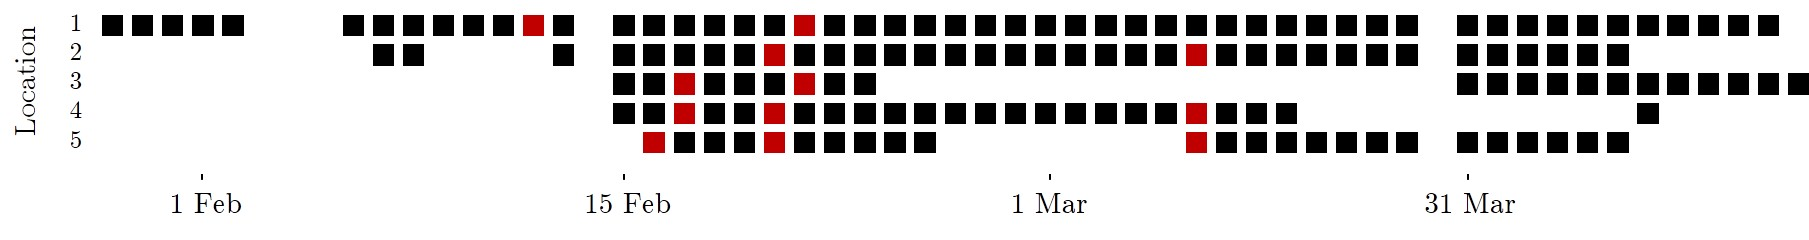
\includegraphics [width=0.90\linewidth] {images/main_schedule.jpeg}
		\caption{Data collection schedule showing the days when sensors were active at their corresponding locations. The red squares show that manual counting of pedestrians was also done on that day.}
		\label{main_schedule}
	\end{center}
\end{figure}

The locations at which the data were collected are shown in Table
\ref{locations-table}. The locations are chosen for their diverse site
conditions and unique sources of noise around the potential location of the
sensors. The position of the sensor at these locations with respect to the
context is shown the Figure \ref{main_signal_strength}. We can see that Location
5 is the `cleanest' with one clear stationary source of noise (phone shop) of
while location 2 is the one with the most complexity with seating area all
around the sensor.  The sensors were operational through out February and March
while manual counts were conducted in these location in half hour sessions on at
least two different days. For the purposes of comparing with ground truth we
just considered the data from sensors which corresponding to the 12 sets of
available manual counts. The schedule of data collection is shown in Figure
\ref{main_schedule}

\begin{figure}
	\centering
	\subfigure[Installation configuration of sensors at the survey locations (not to scale)]{
		\resizebox*{0.46\linewidth}{!}{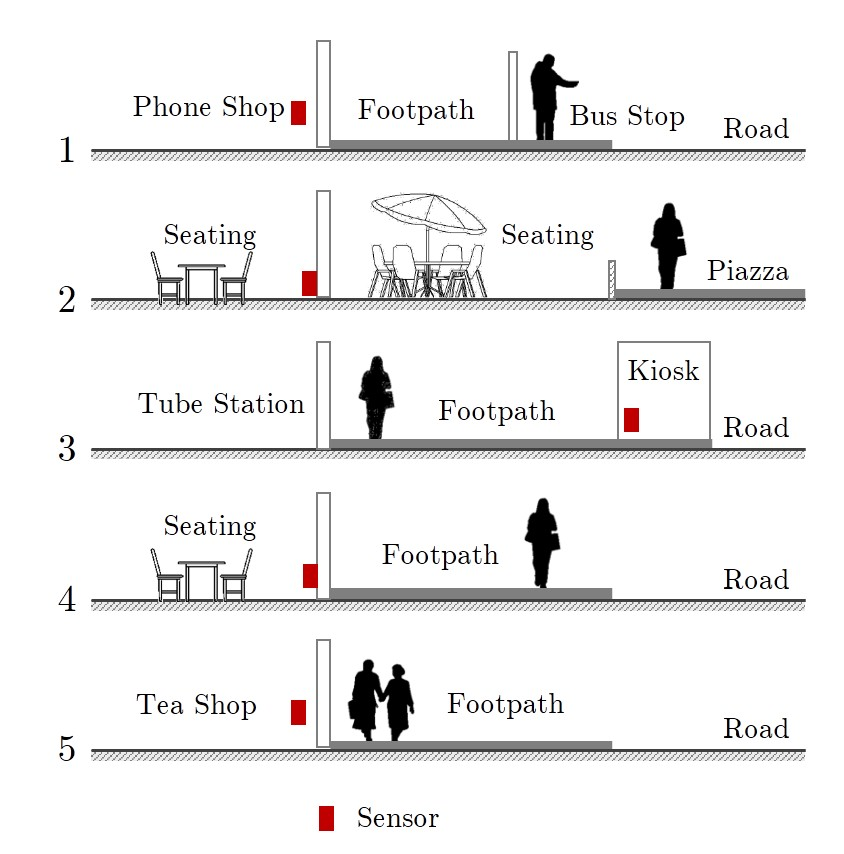
\includegraphics[trim=20 6 20 6,clip]{images/main_configs.jpeg}}}\hspace{20pt}
	\subfigure[Density distribution of signal strength reported in collected probe requests (lower values show higher signal strength)]{
		\resizebox*{0.46\linewidth}{!}{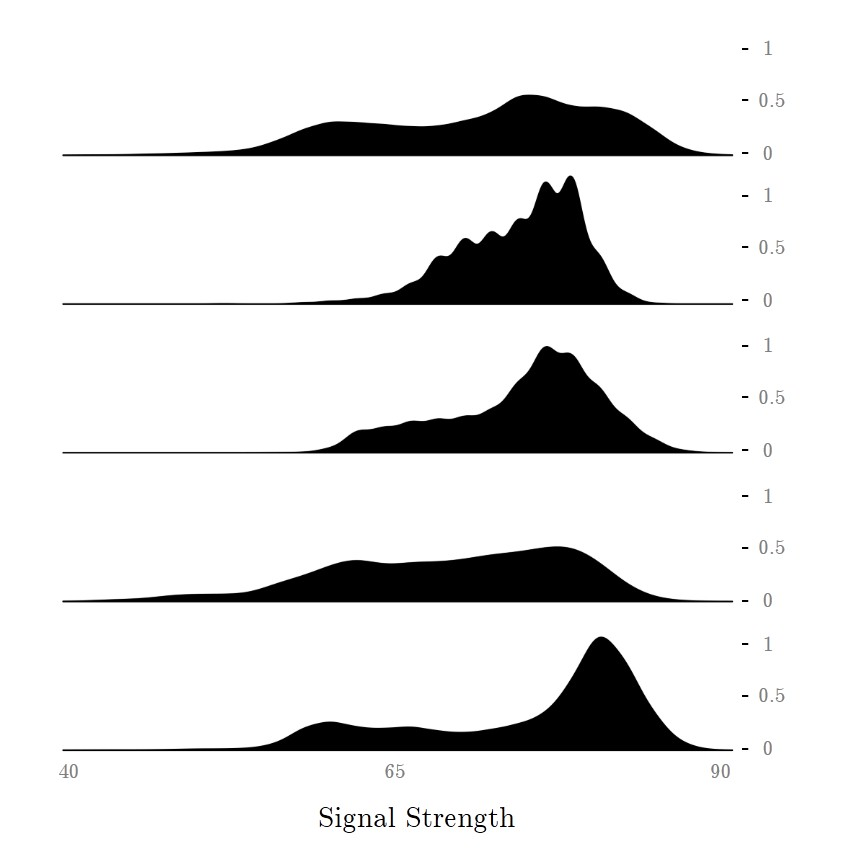
\includegraphics[trim=20 4 25 6,clip]{images/main_signals.jpeg}}}
	\caption{Distribution of signal strengths across locations} \label{main_signal_strength}
\end{figure}

We start by looking at the distribution of the signal strength reported by the
probe requests across the locations. From the density plot shown in Figure
\ref{main_signal_strength} we can see that there is clear relation between the
distribution of the signal strength and the distance and complexity of the
source of noise. We can see that while location 5 shows clean difference between
low and high signal strengths, location 2 is almost normally distributed.
Intuitively we expect that location 2 and 4 must be harder to classify than
location 1 3 and 5.  We run the k-means clustering algorithm and filter out the
probe requests which are randomised and have signal strengths less than the
second break (threshold).  It is important to note that we are dealing with
relative thresholds of signal strengths which can vary with location and time of
the analysis.  We then aggregate then probe requests for every minute by
counting the number of Unique MAC addresses present in every minute. We also
remove devices that dwell around the sensor by removing the MAC addresses which
reappear from within the past hour.  The results of the first stage of filtering
process along with the thresholds are shown in Table \ref{errors_table}.
Confirming our intuition, we see that the location 2 has the most MAPE followed
by location 4 while rest of them have highly reduced MAPE.  It is significant
that this method alone reduces our margin of error by a 50 - 100\% from the raw
counts without any cleaning.  This makes the signal strength filtering quick and
ideal method for practical applications which doesn't require absolute numbers
such as creating large aggregated indexes to show long term trends.  We also see
that the success of the signal strength filtering can be improved significantly
by installing sensors such that the pedestrians and noise are at different
distances from the sensor and are the field of measurement is distinct from the
surroundings however noisy it might be.

We then run the sequence numbers based clustering process on the rest of the
probe requests to reduce the MAPE by almost 50 - 100\% on all the sensors except
for location 3.  Location 3 is an outlier among all the other sensors since it
is the only one with large amount of pedestrians very close to the sensor.  This
may be causing the over filtering caused by the previous process.  We finally
run the calibration process where we calculate the adjustment factors from the
ratio between the manual counts to the counts calculated for the sample period
as shown in Table \ref{errors_table}.  We the use them to adjust the counts to
achieve a MAPE ranging from 10 - 50\%. We can see that the sensors with people
moving right next to them tend to under-count with our methodology while sensors
with seating next to them tend to over-count significantly. However, using the
filtering process, we can reduce the error to almost 10\% closer to that of the
ground truth.

\begin{table}
	\tbl{Results of footfall estimation at each location as Mean Absolute Percentage Error (MAPE) after each step of the filtering process}
	{\begin{tabular}{ccccccc} 
		\toprule
			Sensor & Signal strength & Adjustment & MAPE & MAPE after & MAPE after & MAPE of\\
			& threshold & factor & without any & filtering signal & filtering sequence & final adjusted\\
			& (-dBm) & &  cleaning (\%) & strength (\%) & numbers (\%) & counts (\%)\\
		 \midrule
			1 & -70 & 1.25 & 259 &  22 & -13 &  9 \\
			2 & -74 & 0.51 & 928 & 396 & 206 & 55 \\
			3 & -72 & 1.60 &  87 & -19 & -31 & 10 \\
			4 & -70 & 0.88 & 498 & 142 &  52 & 33 \\
			5 & -72 & 0.80 & 473 &  84 &  38 & 11 \\
		 \bottomrule
	\end{tabular}}
	\label{errors_table}
\end{table}

\begin{figure}
	\begin{center}
		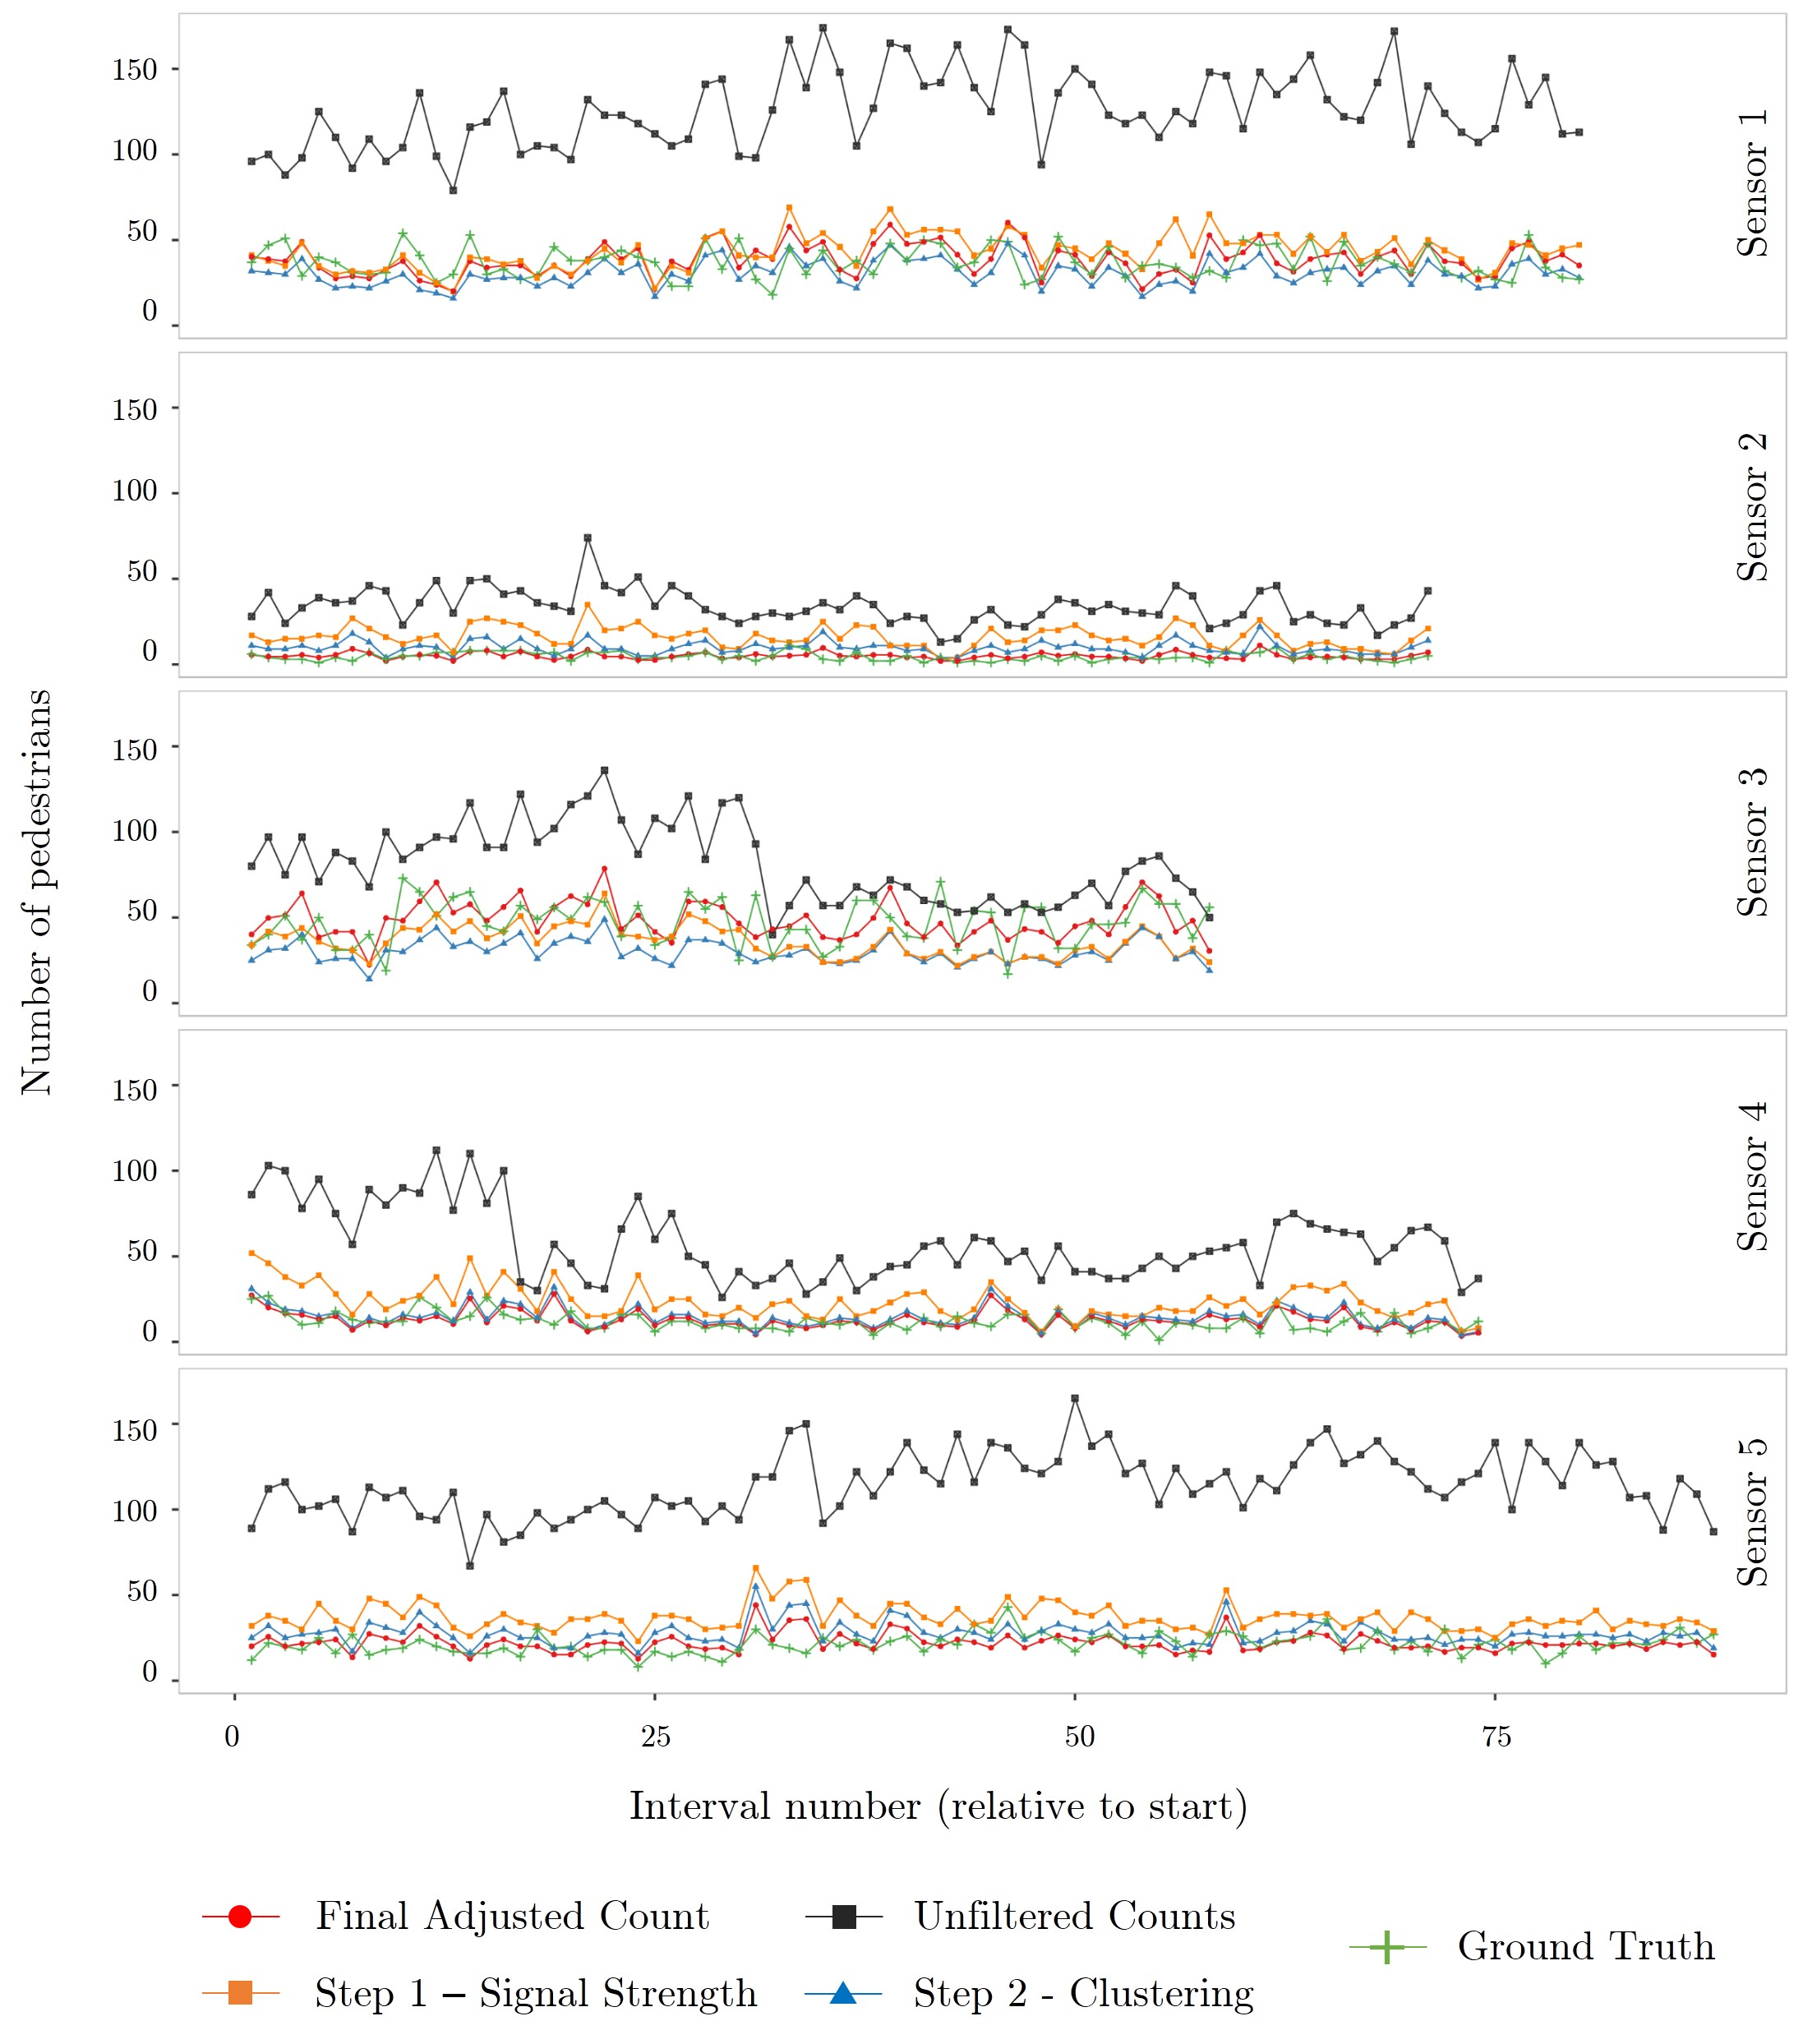
\includegraphics [width=\linewidth,trim=6 6 6 6,clip] {images/main_comparison.jpeg}
		\caption{Comparison of the filtering process with the ground truth in all the locations.}
		\label{main_comparison}
	\end{center}
\end{figure}

\begin{figure}
	\begin{center}
		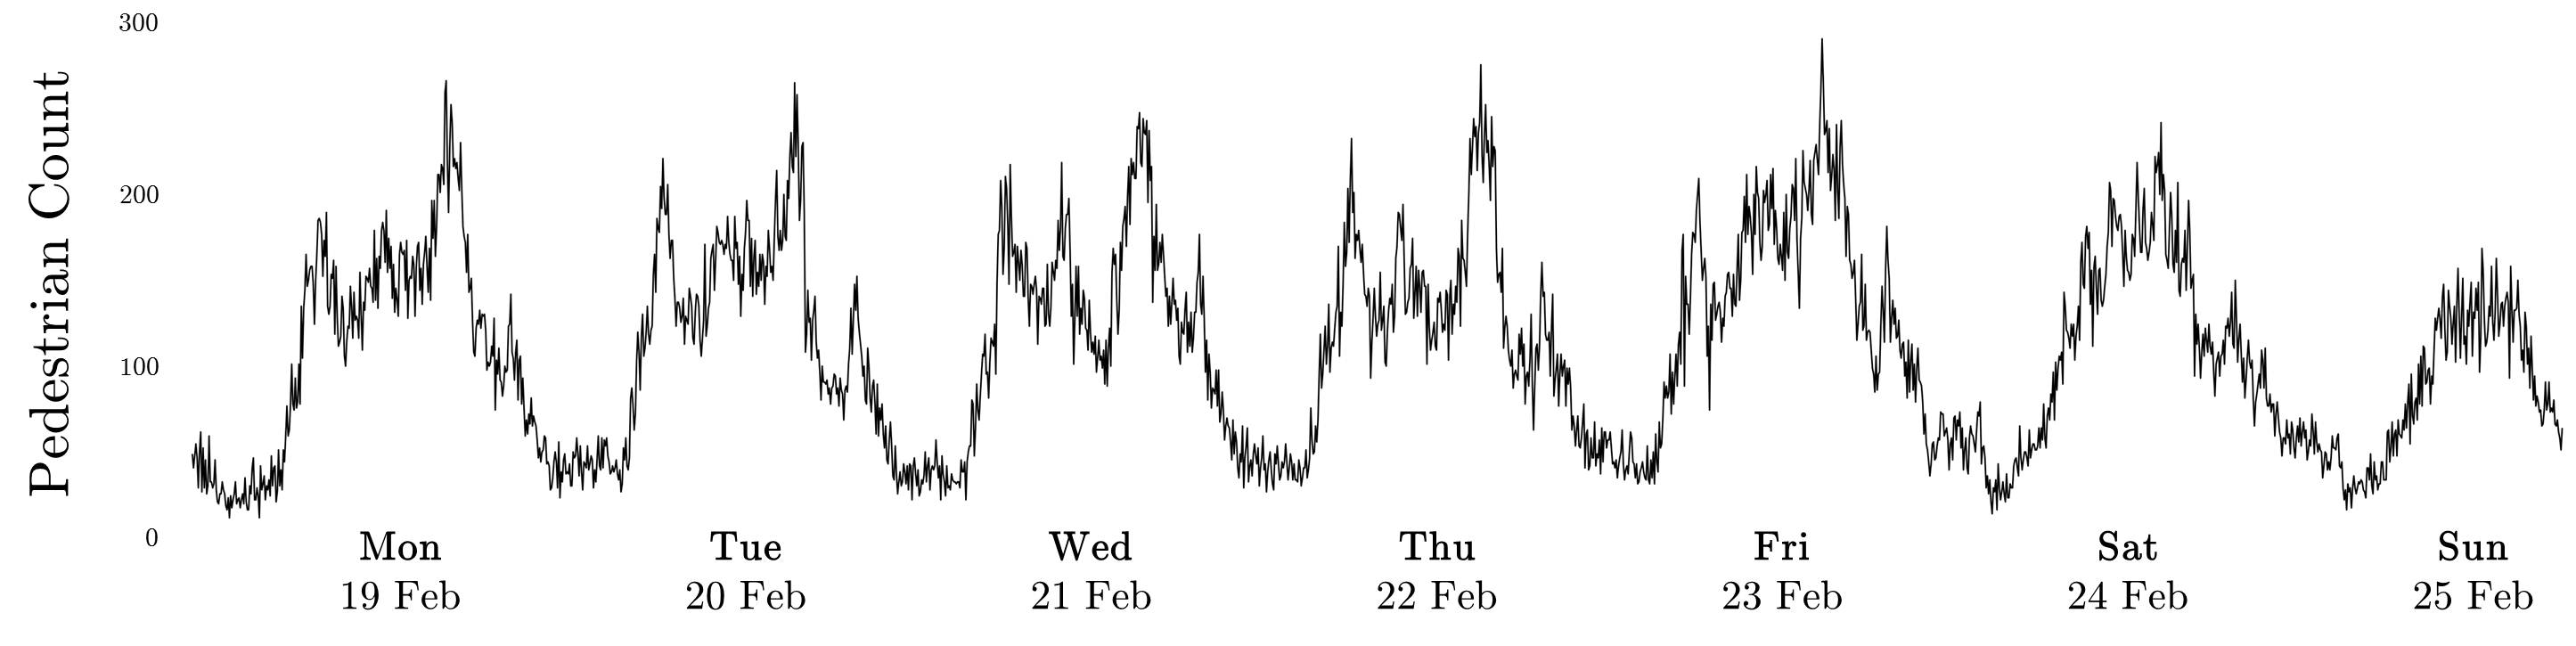
\includegraphics [width=\linewidth] {images/main_footfall.jpeg}
		\caption{A week of pedestrian footfall at the Strand, London collected by the methodology. The counts are aggregated for 5 minute intervals.}
		\label{main_study_counts}
	\end{center}
\end{figure}
